\documentclass{rapportECL}
\usepackage{lipsum}
\title{Rapport ECL - Template} %Titre du fichier

\begin{document}

%----------- Informations du rapport ---------

\titre{TD Thermique1} %Titre du fichier .pdf
%Nom de la UE
\sujet{THERMIQUE S9} %Nom du sujet

\enseignant{Philippe \textsc{BERTRAND}} %Nom de l'enseignant

\eleves{Kévin \textsc{TONGUE} }\\
	%Nom des élèves

%----------- Initialisation -------------------
        
\fairemarges %Afficher les marges
\fairepagedegarde %Créer la page de garde
\tabledematieres %Créer la table de matières

%------------ Corps du rapport ----------------



%------------- Commandes utiles ----------------


%------- Pour insérer et citer une équation --------------





\section*{Résolution Détaillée des Problèmes de Transfert Thermique (TD N1)}

\subsection*{1. Problème de la Fenêtre à Simple Vitrage (Example 17-2)}
\subsubsection*{Données}
\begin{itemize}
    \item Dimensions : $H=0.8 \ \text{m}$, $W=1.5 \ \text{m}$. Aire $A = 1.2 \ \text{m}^2$. 
    \item Épaisseur du verre : $L = 0.008 \ \text{m}$. Conductivité : $k = 0.78 \ \text{W/m}\cdot^\circ\text{C}$. 
    \item Températures : $T_{\infty 1} = 20^\circ\text{C}$, $T_{\infty 2} = -10^\circ\text{C}$. 
    \item Coefficients de convection : $h_1 = 10 \ \text{W/m}^2\cdot^\circ\text{C}$, $h_2 = 40 \ \text{W/m}^2\cdot^\circ\text{C}$. 
\end{itemize}

\subsubsection*{Résistances Thermiques}
Le transfert de chaleur est en série : Convection interne $\rightarrow$ Conduction $\rightarrow$ Convection externe.
\begin{align*}
    R_{\text{conv}, 1} &= \frac{1}{h_1 A} = \frac{1}{(10)(1.2)} = 0.08333 \ ^\circ\text{C/W} \\
    R_{\text{verre}} &= \frac{L}{k A} = \frac{0.008}{(0.78)(1.2)} = 0.00855 \ ^\circ\text{C/W} \\
    R_{\text{conv}, 2} &= \frac{1}{h_2 A} = \frac{1}{(40)(1.2)} = 0.02083 \ ^\circ\text{C/W}
\end{align*}
Résistance totale :
$$R_{\text{total}} = R_{\text{conv}, 1} + R_{\text{verre}} + R_{\text{conv}, 2} = 0.08333 + 0.00855 + 0.02083 = 0.11271 \ ^\circ\text{C/W}$$

\subsubsection*{Taux de Transfert de Chaleur ($\dot{Q}$)}
$$\dot{Q} = \frac{T_{\infty 1} - T_{\infty 2}}{R_{\text{total}}} = \frac{20 - (-10)}{0.11271} = \frac{30}{0.11271} = 266.17 \ \text{W}$$
Le taux de transfert de chaleur est de $\mathbf{266.17 \ \text{W}}$.

\subsubsection*{Température de la Surface Intérieure ($T_1$)}
$$\dot{Q} = \frac{T_{\infty 1} - T_1}{R_{\text{conv}, 1}} \implies T_1 = T_{\infty 1} - \dot{Q} \times R_{\text{conv}, 1}$$
$$T_1 = 20 - (266.17) \times (0.08333) = 20 - 22.18 = -2.18 \ ^\circ\text{C}$$
La température de la surface intérieure est $\mathbf{-2.18 \ ^\circ\text{C}}$.

\vspace{0.5cm}
\hrule
\vspace{0.5cm}

\subsection*{2. Problème de la Fenêtre à Double Vitrage (Example 17-3)}
\subsubsection*{Données}
\begin{itemize}
    \item $A = 1.2 \ \text{m}^2$. $T_{\infty 1}=20^\circ\text{C}$, $T_{\infty 2}=-10^\circ\text{C}$, $h_1=10$, $h_2=40$. [cite: 14, 15]
    \item Verre (G) : $L_G = 0.004 \ \text{m}$, $k_G = 0.78 \ \text{W/m}\cdot^\circ\text{C}$. 
    \item Air (A) : $L_A = 0.010 \ \text{m}$, $k_A = 0.026 \ \text{W/m}\cdot^\circ\text{C}$. 
\end{itemize}

\subsubsection*{Résistances Thermiques}
Le circuit comporte 5 résistances en série : $R_{\text{conv}, 1}$, $R_{\text{G}, 1}$, $R_{\text{air}}$, $R_{\text{G}, 2}$, $R_{\text{conv}, 2}$.
\begin{align*}
    R_{\text{conv}, 1} &= 0.08333 \ ^\circ\text{C/W} \\
    R_{\text{conv}, 2} &= 0.02083 \ ^\circ\text{C/W} \\
    R_{\text{G}} &= \frac{L_G}{k_G A} = \frac{0.004}{(0.78)(1.2)} = 0.00427 \ ^\circ\text{C/W} \\
    R_{\text{air}} &= \frac{L_A}{k_A A} = \frac{0.010}{(0.026)(1.2)} = 0.32051 \ ^\circ\text{C/W}
\end{align*}
Résistance totale :
$$R_{\text{total}} = 0.08333 + 0.00427 + 0.32051 + 0.00427 + 0.02083 = 0.43321 \ ^\circ\text{C/W}$$

\subsubsection*{Taux de Transfert de Chaleur ($\dot{Q}$)}
$$\dot{Q} = \frac{T_{\infty 1} - T_{\infty 2}}{R_{\text{total}}} = \frac{30}{0.43321} = 69.25 \ \text{W}$$
Le taux de transfert de chaleur est de $\mathbf{69.25 \ \text{W}}$.

\subsubsection*{Température de la Surface Intérieure ($T_1$)}
$$T_1 = T_{\infty 1} - \dot{Q} \times R_{\text{conv}, 1} = 20 - (69.25) \times (0.08333) = 20 - 5.77 = 14.23 \ ^\circ\text{C}$$
La température de la surface intérieure est $\mathbf{14.23 \ ^\circ\text{C}}$.

\vspace{0.5cm}
\hrule
\vspace{0.5cm}

\subsection*{3. Problème du Tuyau de Vapeur Isolé (Example 17-8)}
\subsubsection*{Données et Rayons}
\begin{itemize}
    \item $T_{\infty 1} = 320^\circ\text{C}$, $T_{\infty 2} = 5^\circ\text{C}$. $h_1 = 60$, $h_2 = 18$. [cite: 28, 30]
    \item Tuyau : $k_p=80$. $r_1 = 0.025 \ \text{m}$, $r_2 = 0.0275 \ \text{m}$. 
    \item Isolation : $k_{\text{isol}}=0.05$. $r_3 = r_2 + 0.17 = 0.1975 \ \text{m}$. 
\end{itemize}

\subsubsection*{Résistances Thermiques par Unité de Longueur ($R'$)}
\begin{align*}
    R'_{\text{conv}, 1} &= \frac{1}{h_1 (2\pi r_1)} = \frac{1}{60 \times 2\pi \times 0.025} = 0.10610 \ \text{m}\cdot^\circ\text{C/W} \\
    R'_{\text{tuyau}} &= \frac{\ln(r_2/r_1)}{2\pi k_p} = \frac{\ln(0.0275/0.025)}{2\pi \times 80} = 0.00023 \ \text{m}\cdot^\circ\text{C/W} \\
    R'_{\text{isol}} &= \frac{\ln(r_3/r_2)}{2\pi k_{\text{isol}}} = \frac{\ln(0.1975/0.0275)}{2\pi \times 0.05} = 6.4475 \ \text{m}\cdot^\circ\text{C/W} \\
    R'_{\text{conv}, 2} &= \frac{1}{h_2 (2\pi r_3)} = \frac{1}{18 \times 2\pi \times 0.1975} = 0.04461 \ \text{m}\cdot^\circ\text{C/W}
\end{align*}
Résistance totale :
$$R'_{\text{total}} = 0.10610 + 0.00023 + 6.4475 + 0.04461 = 6.59844 \ \text{m}\cdot^\circ\text{C/W}$$

\subsubsection*{Taux de Perte de Chaleur par Unité de Longueur ($\dot{Q}/L$)}
$$\frac{\dot{Q}}{L} = \frac{T_{\infty 1} - T_{\infty 2}}{R'_{\text{total}}} = \frac{320 - 5}{6.59844} = \frac{315}{6.59844} = 47.74 \ \text{W/m}$$
Le taux de perte de chaleur est de $\mathbf{47.74 \ \text{W/m}}$.

\subsubsection*{Chutes de Température}
\begin{itemize}
    \item Chute à travers le tuyau : $\Delta T_{\text{tuyau}} = \frac{\dot{Q}}{L} R'_{\text{tuyau}} = 47.74 \times 0.00023 = \mathbf{0.011 \ ^\circ\text{C}}$ 
    \item Chute à travers l'isolation : $\Delta T_{\text{isol}} = \frac{\dot{Q}}{L} R'_{\text{isol}} = 47.74 \times 6.4475 = \mathbf{307.82 \ ^\circ\text{C}}$ 
\end{itemize}

\vspace{0.5cm}
\hrule
\vspace{0.5cm}

\subsection*{4. Problème du Mur Composite avec Génération de Chaleur (Example 3.7)}
\subsubsection*{Données}
\begin{itemize}
    \item Matériau A : $\dot{q} = 1.5 \times 10^6 \ \text{W/m}^3$, $k_A=75$, $L_A=0.05 \ \text{m}$. 
    \item Matériau B : $\dot{q}_B=0$, $k_B=150$, $L_B=0.02 \ \text{m}$. 
    \item Condition Convective : $T_{\infty}=30^\circ\text{C}$, $h=1000 \ \text{W/m}^2\cdot\text{K}$. 
    \item Condition Isolée : $\left.\frac{dT}{dx}\right|_{x=0} = 0$. 
\end{itemize}

\subsubsection*{Flux Thermique Stationnaire ($q''$)}
Le flux généré dans A doit quitter la paroi :
$$q'' = \dot{q} L_A = (1.5 \times 10^6 \ \text{W/m}^3) \times (0.05 \ \text{m}) = 75,000 \ \text{W/m}^2$$

\subsubsection*{Détermination de la Température $T_2$ (Surface Refroidie)}
Le flux est perdu par convection à $x=L_A+L_B$:
$$q'' = h (T_2 - T_{\infty}) \implies T_2 = T_{\infty} + \frac{q''}{h}$$
$$T_2 = 30 + \frac{75,000}{1000} = 30 + 75 = \mathbf{105 \ ^\circ\text{C}}$$ 

\subsubsection*{Détermination de la Température $T_1$ (Interface A/B)}
Le flux est conduit à travers B ($L_B=0.02 \ \text{m}$):
$$q'' = k_B \frac{T_1 - T_2}{L_B} \implies T_1 = T_2 + \frac{q'' L_B}{k_B}$$
$$T_1 = 105 + \frac{(75,000)(0.02)}{150} = 105 + 10 = \mathbf{115 \ ^\circ\text{C}}$$

\subsubsection*{Détermination de la Température $T_0$ (Surface Isolée)}
L'équation de conduction dans A, $T(x) = T_0 - \frac{\dot{q}}{2 k_A} x^2$, évaluée à $x=L_A$:
$$T_0 = T_1 + \frac{\dot{q} L_A^2}{2 k_A}$$
$$T_0 = 115 + \frac{(1.5 \times 10^6) \times (0.05)^2}{2 \times 75} = 115 + 25 = \mathbf{140 \ ^\circ\text{C}}$$ 

\subsubsection*{Distribution de Température (Esquisse)}
\begin{enumerate}
    \item $0 \le x \le L_A$ (Matériau A) : Parabolique, maximum en $T_0=140^\circ\text{C}$ ($x=0$), décroissant à $T_1=115^\circ\text{C}$ ($x=L_A$).
    \item $L_A \le x \le L_A+L_B$ (Matériau B) : Linéaire, décroissant de $T_1=115^\circ\text{C}$ à $T_2=105^\circ\text{C}$ ($x=L_A+L_B$).
\end{enumerate}
\begin{figure}[!H]
    \centering
    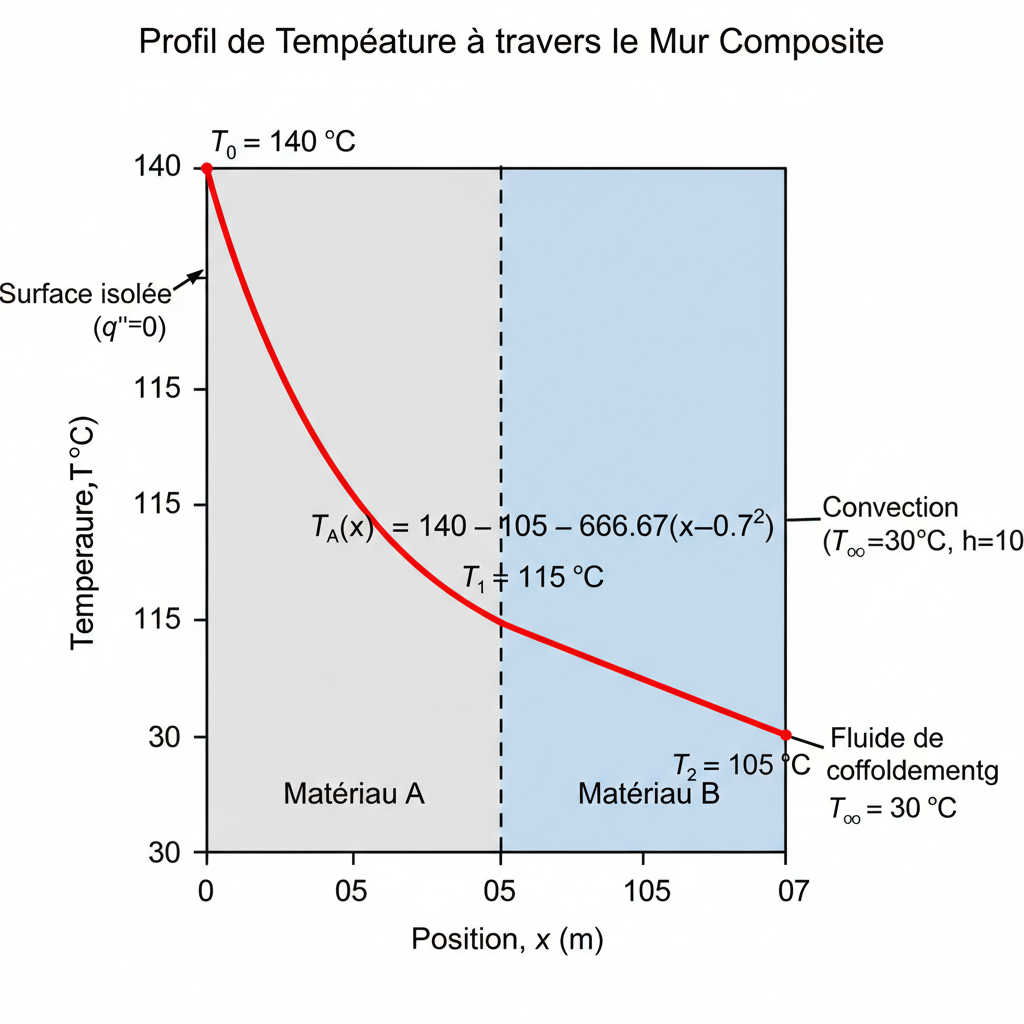
\includegraphics[width=0.5\linewidth]{image.png}
    \caption{Profil de température}
    \label{fig:placeholder}
\end{figure}
\end{document}

